%%%%%%%%%%%%%%%%%%%%%%%%%%%

%%%%%%%%%%%%%%%%%%%%%%%%%%%_________________CHAPTERTHREE_________________%%%%%%%%%%%%%%%%%%%%%%%%%%%

%%%%%%%%%%%%%%%%%%%%%%%%%%%

\chapter{Chapter 3 Supplemental Information}
\label{sec:app3}
\clearpage
\section{Supplemental Figures}

%Supplemental Figure 1: Cell counts in NB 
\begin{figure}[h!]
  \centering
    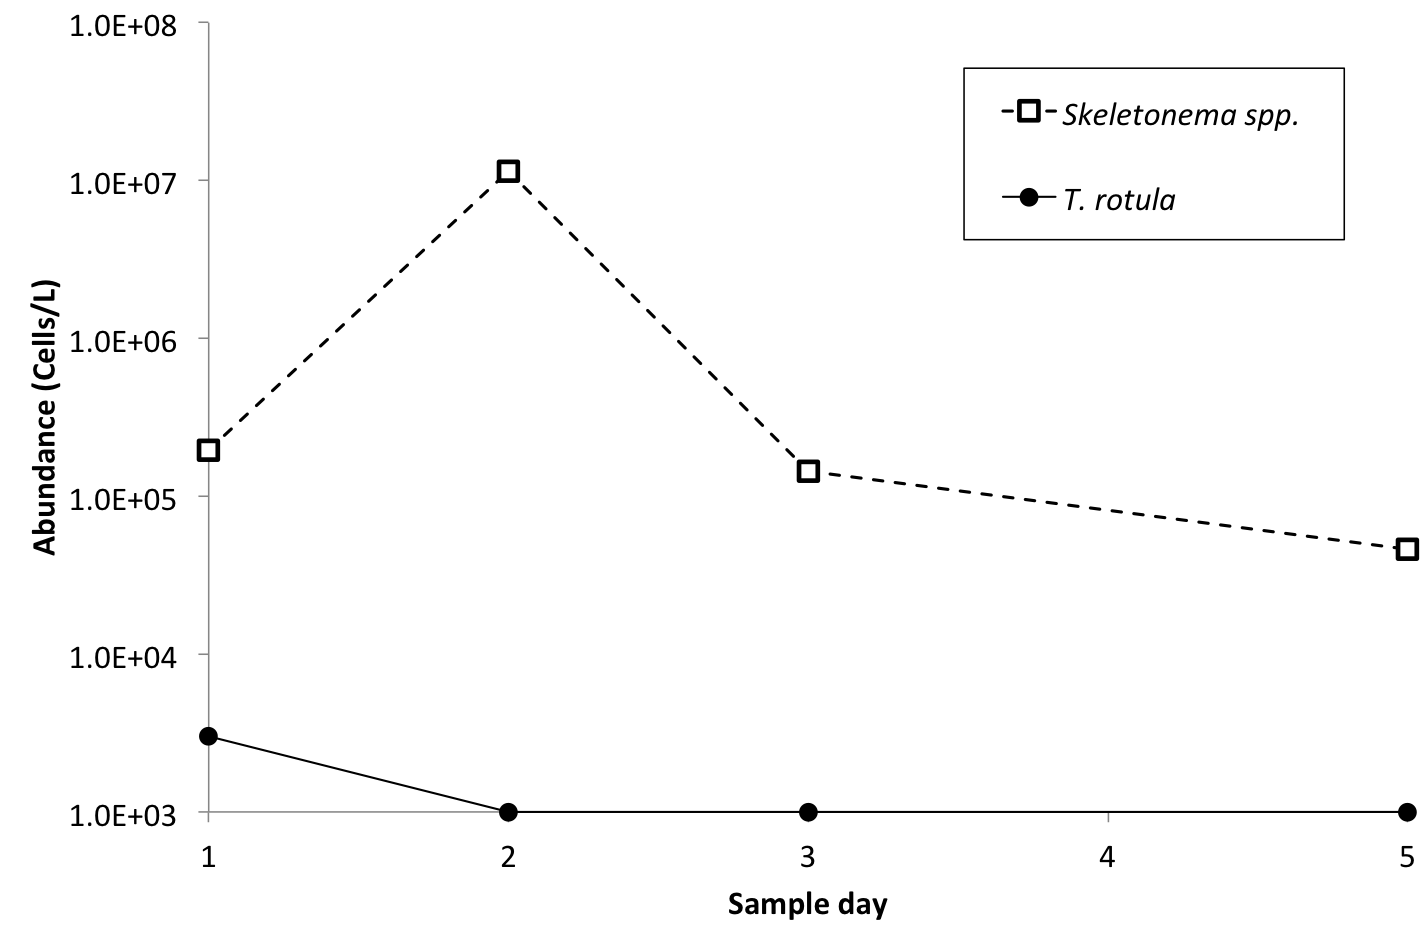
\includegraphics[width=1\textwidth]{Images/C3_SFigure1_CellCounts.png}
    \caption[Cell counts in Narragansett Bay during the spring of 2012]{Abundance estimation from cell counts of \textit{Skeletonema} spp. and \textit{T. rotula} across the five sample points during the spring of 2012. }
  \label{fig:a3f1}
\end{figure}


%Supplemental Figure 2: KEGG linear correlation
\begin{figure}[p!]
  \centering
    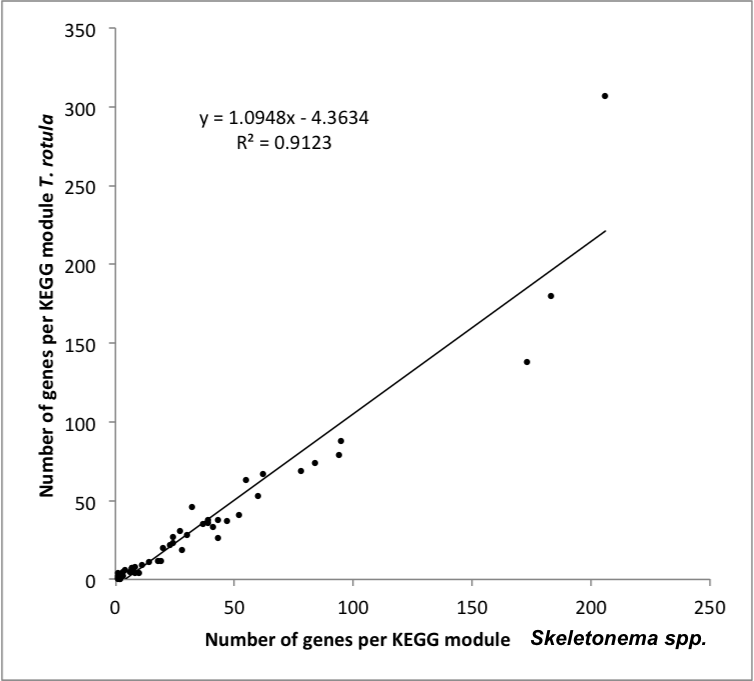
\includegraphics[width=1\textwidth]{Images/C3_SFigure2_KEGGModuleGeneContent2.png}
    \caption[Comparison of KEGG module content between \textit{Skeletonema} spp. and \textit{T. rotula} ]{Total number of genes assigned to each KEGG module for \textit{Skeletonema} spp. and \textit{T. rotula}.}
  \label{fig:a3f2}
\end{figure}


%Supplemental Figure 3: Hierarchical clustering of S and T across time
\begin{figure}[p!]
  \centering
    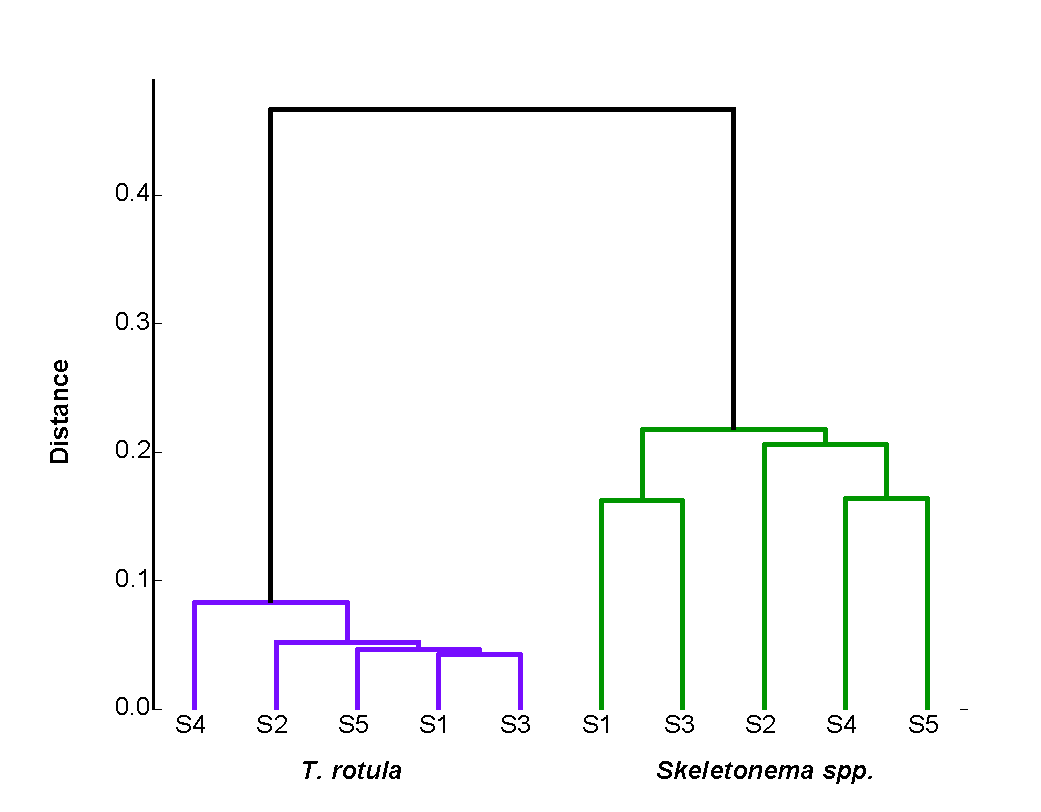
\includegraphics[width=1\textwidth]{Images/C3_SFigure3_Dendrogram.pdf}
    \caption[Hierarchical clustering of QMF signatures across species and samples]{Dendrogram depicting hierarchical clustering of samples based on relative expression of KEGG modules (Figure 2) across the five samples S1-S5 for \textit{Skeletonema} spp. and \textit{T. rotula}.}
  \label{fig:a3f3}
\end{figure}

%Supplemental Figure 4: Stable gene expression across time
\begin{figure}[p!]
  \centering
    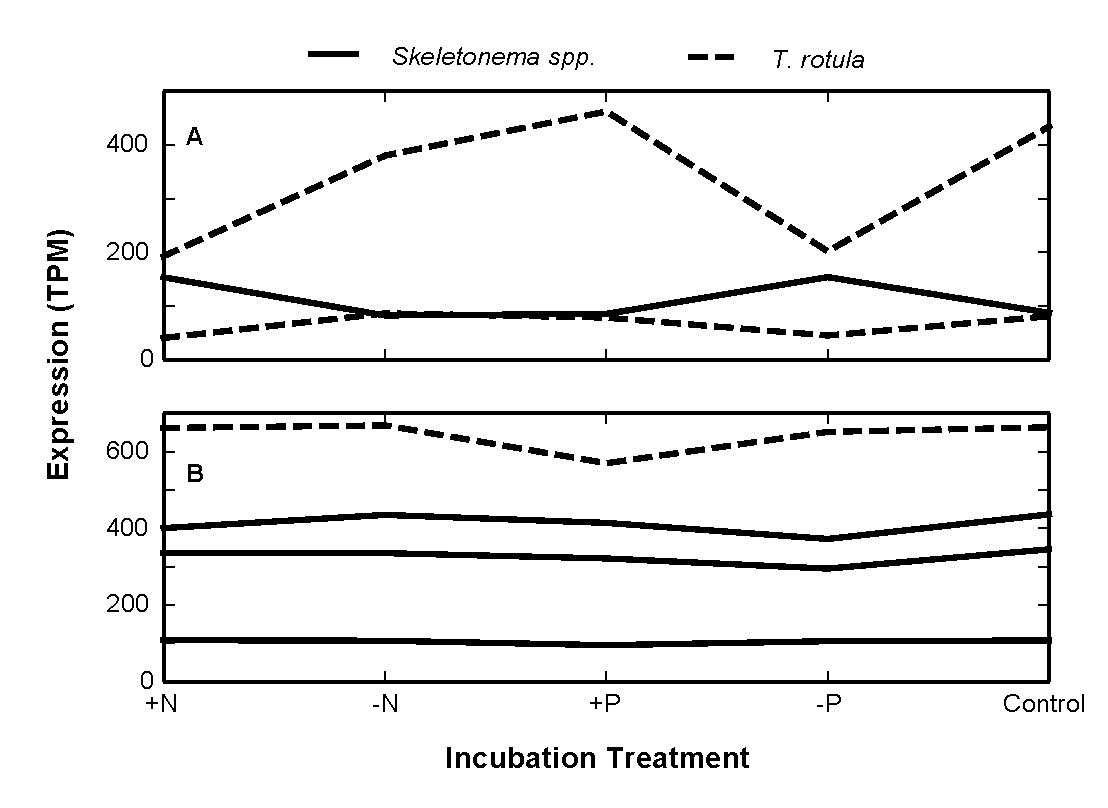
\includegraphics[width=1\textwidth]{Images/C3_SFigure4_StableGenePlot_wActin.pdf}
    \caption[Expression of stable reference genes in the field]{Expression of stable reference genes identified based on literature and statistical parsing in nutrient amendment incubation. (A) The expression in tags per million ($TPM$) of stable reference genes identified in \textit{T. rotula} (dashed line) and \textit{Skeletonema} spp.  (solid lines) based on homology (e-value < 1e-5) to a known reference genes in \textit{T. pseudonana}, ACT1 (Thaps\_25772), in nutrient incubations. (B) Also shown are reference genes identified in the incubation experiments, using statistical analysis of sequence counts \citep{Alexander2012, Wu2010}, and nutrient incubations }
  \label{fig:a3f4}
\end{figure}

%Supplemental Figure 5: RR gene composition
\begin{figure}[p!]
  \centering
    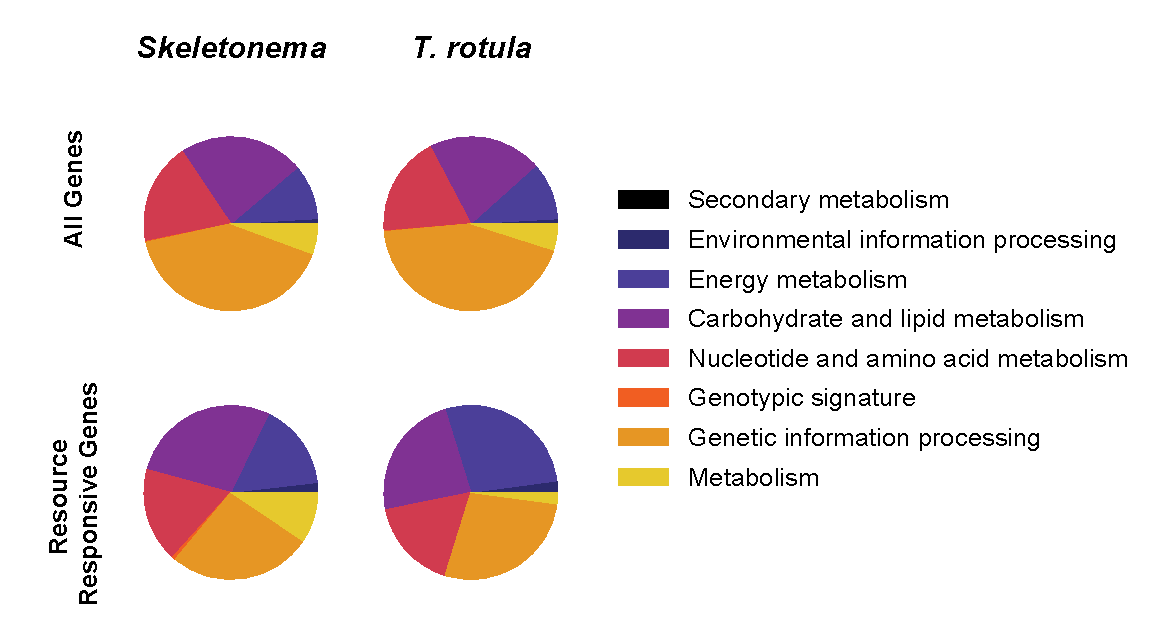
\includegraphics[width=1\textwidth]{Images/C3_SFigure5_RR_All_Genes_Pie.pdf}
    \caption[Functional composition of the reference transcriptome and resource-responsive gene sets]{Functional composition of the reference transcriptome and resource-responsive (RR) gene subset for \textit{T. rotula} and \textit{Skeletonema} spp. (A) RR gene sets were identified through cross comparison of like-nutrient incubations (i.e. +N vs. -N and +P vs. -P), using ASC (fold change = 2, post-$p > 0.95$). The relative functional categorization of the reference transcriptomes and RR gene set for \textit{T. rotula} and \textit{Skeletonema} spp. based on KEGG ontology as assigned by KAAS is depicted at the module-level.}
  \label{fig:a3f5}
\end{figure}

%Supplemental Figure 6: Expression of nitrate reductase

\begin{figure}[p!]
  \centering
    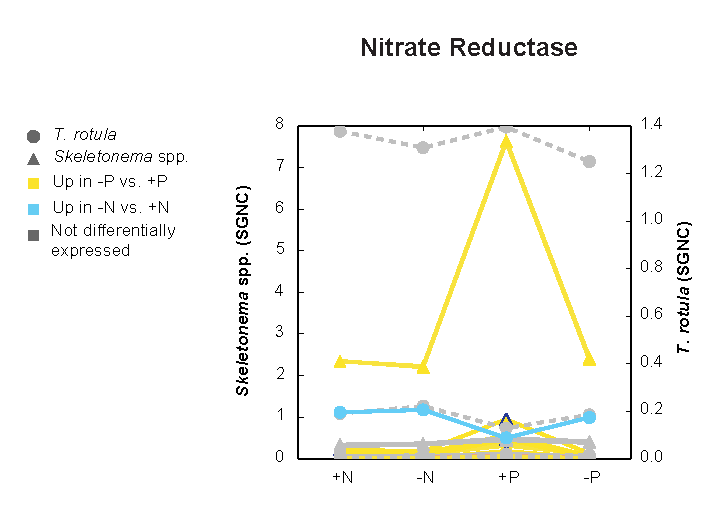
\includegraphics[width=1\textwidth]{Images/C3_SFigure6_SGNC_NitrateReductase.pdf}
    \caption[Relative expression of nitrate reducatses across incubation experiments]{The relative expression in stable gene normalized counts ($SGNC$) of the assimilatory nitrate reductase gene cluster across the incubation experiment treatments. Significance of regulation between the treatments is denoted by the color of the line; organisms are denoted by the shapes of the marker.}
  \label{fig:a3f6}
\end{figure}

%Supplemental Figure 7: Cluster Analysis


\begin{figure}[p!]
  \centering
    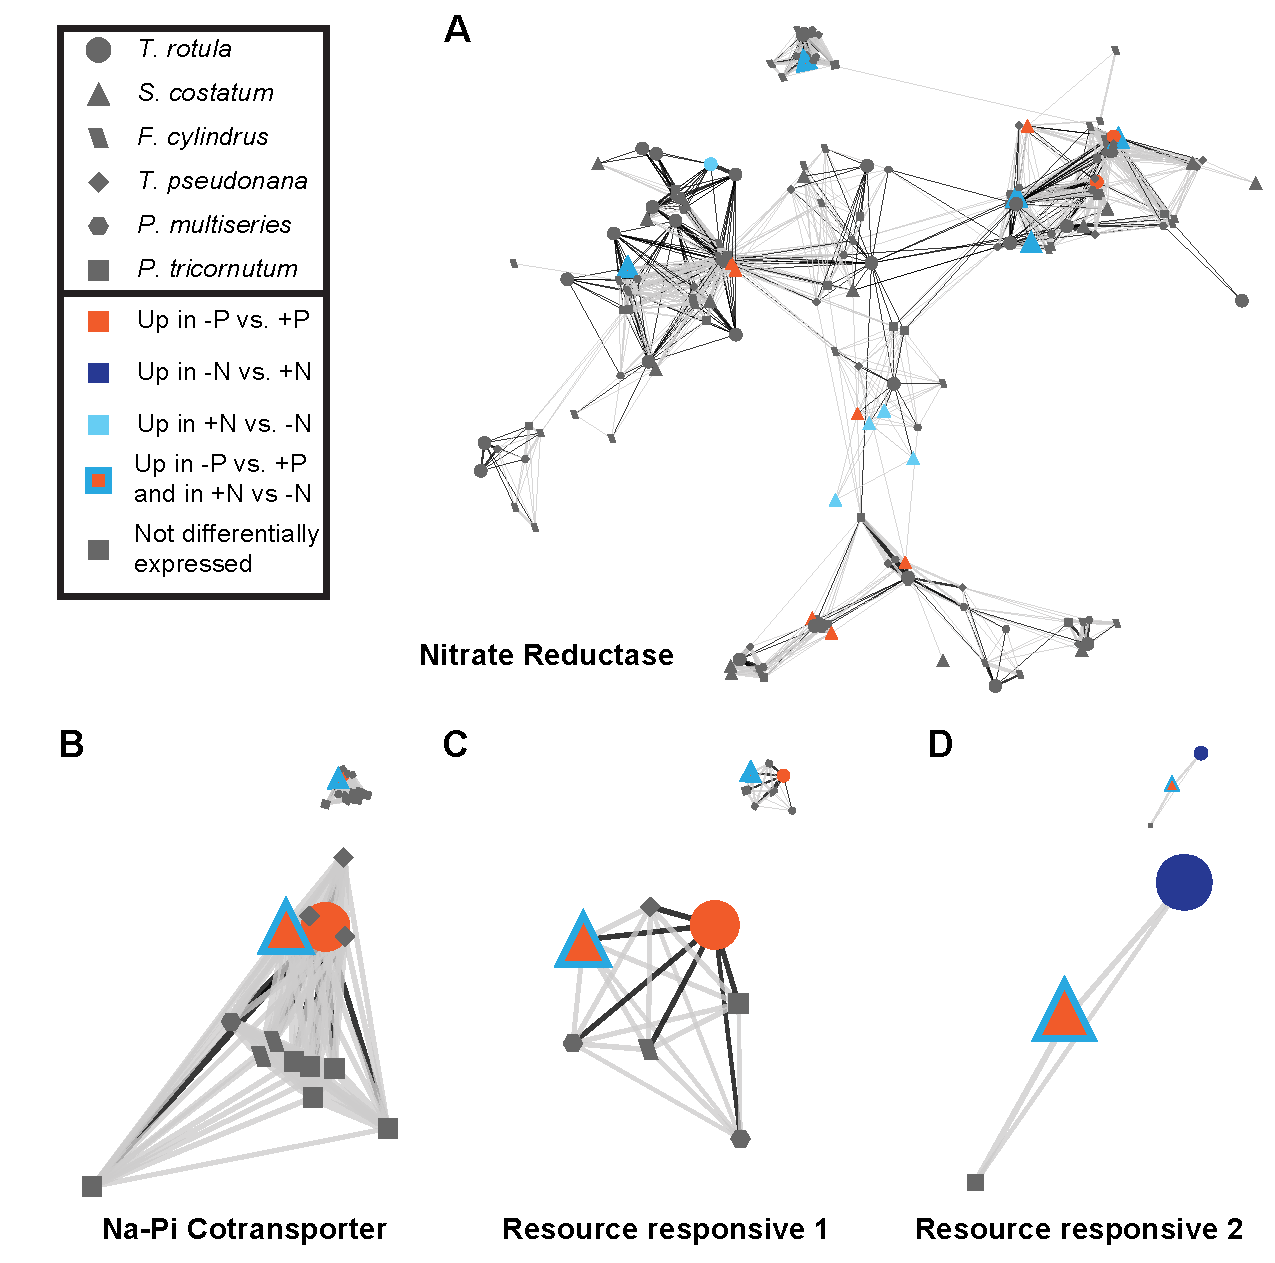
\includegraphics[width=1\textwidth]{Images/C3_SFigure7_ClusterAnalysis_v5.pdf}
    \caption[Gene cluster analysis of nutrient-responsive genes]{Gene cluster known nutrient-responsive genes in \textit{T. pseudonana}: (A) assimilatory nitrate reductase and (B) sodium-phosphate cotransporter and novel resource-responsive (RR) gene families: (C) RR1 and (D) RR2. Transcripts from the transcriptomes of \textit{T. rotula} and \textit{Skeletonema} spp. were clustered based upon relative homology with available diatom genomes: \textit{F. cylindrus}, \textit{P. tricornitum}, \textit{P. multiseries}, and \textit{T. pseudonana}. Symbols indicate different species, while color indicates regulation in the field incubation experiments. Two nodes within a gene cluster are connected by an edge if they share a homologous protein (reciprocal BLAST hit with a minimum of 1e-5 score and minimum 20\% identity). Gene clusters are visualized using an edge-weighted spring-embedded model based on e-value, meaning that genes that are closer together are more similar. The width of the line correlates to the magnitude of the e-value, with lower e-values represented by thicker lines and higher e-values represented by thinner lines.}
  \label{fig:a3f7}
\end{figure}




%Supplemental Figure 8: NaPI Example
\begin{figure}[p!]
  \centering
    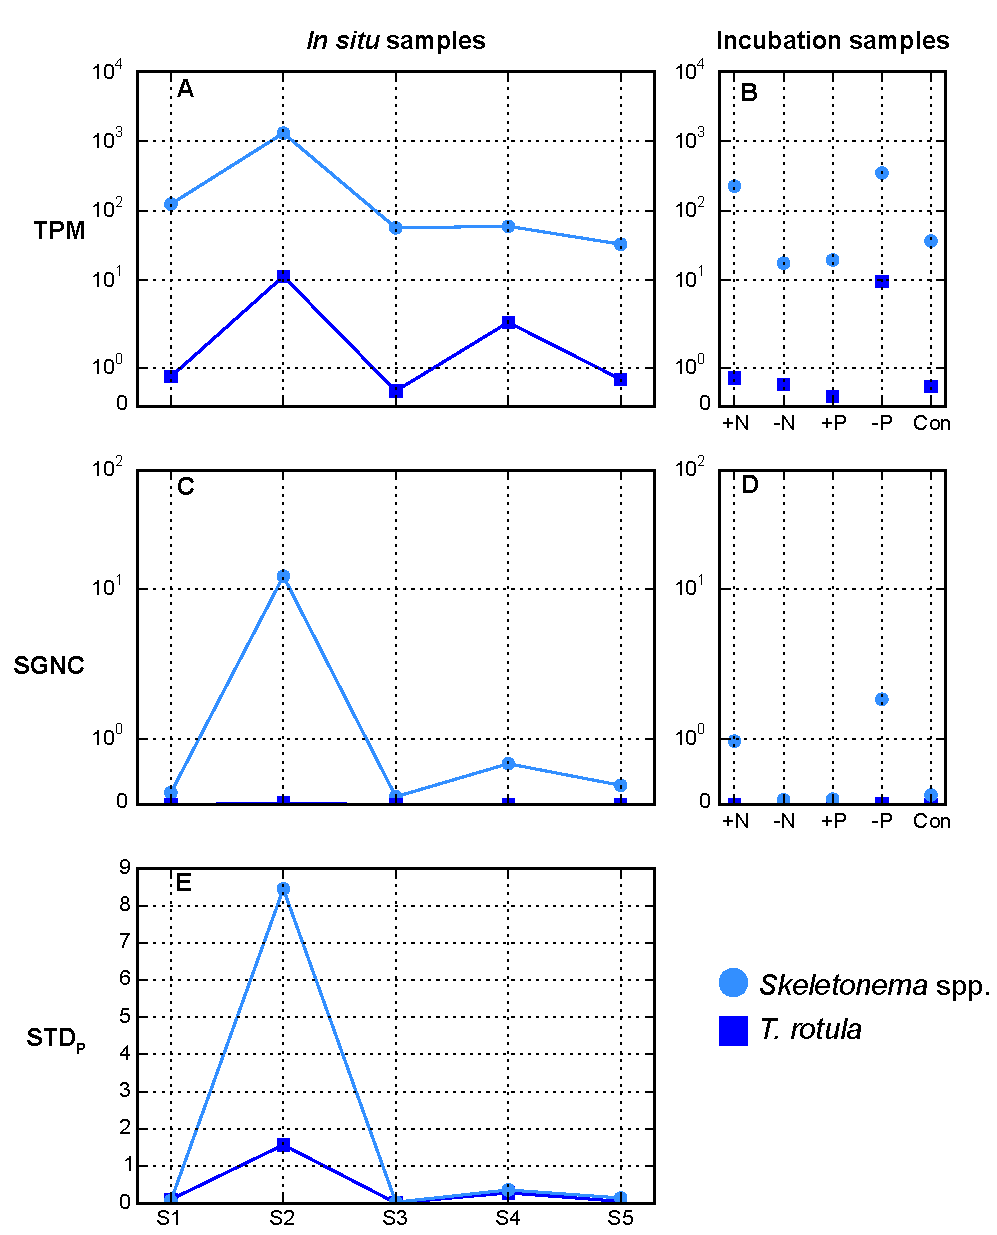
\includegraphics[width=.8\textwidth]{Images/C3_STDP_Steps_NaPi.pdf}
    \caption[Expression of sodium phosphate cotransporter as measured in $TPM$, $SGNC$, and $STD_P$]{The expression of a sodium phosphate cotransporter (NPT) gene family for \textit{Skeletonema} spp. and \textit{T. rotula} as measured in tags per million ($TPM$), stable gene normalized count ($SGNC$), and standardized transcriptional differentiation score for P ($STD_P$). The $TPM$ (A, B) and $SGNC$ (C, D) of the NPT gene family is plotted for \textit{Skeletonema} spp., light blue circles, and \textit{T. rotula}, dark blue squares, both in the \textit{in situ} samples S1-5 (A, C) and the incubation treatments (B, D). The $STD_P$, which contextualizes the expression of a gene in the field relative to expression in the +P and -P treatments, is shown for the five \textit{in situ} samples (E).} 
  \label{fig:a3f8}
\end{figure}


%Supplemental Figure 9: Histogram
\begin{landscape}
   \centering
   \null         %%<---- this is needed
   \vfill        %%<-----here

	\begin{figure}
  	\centering
    	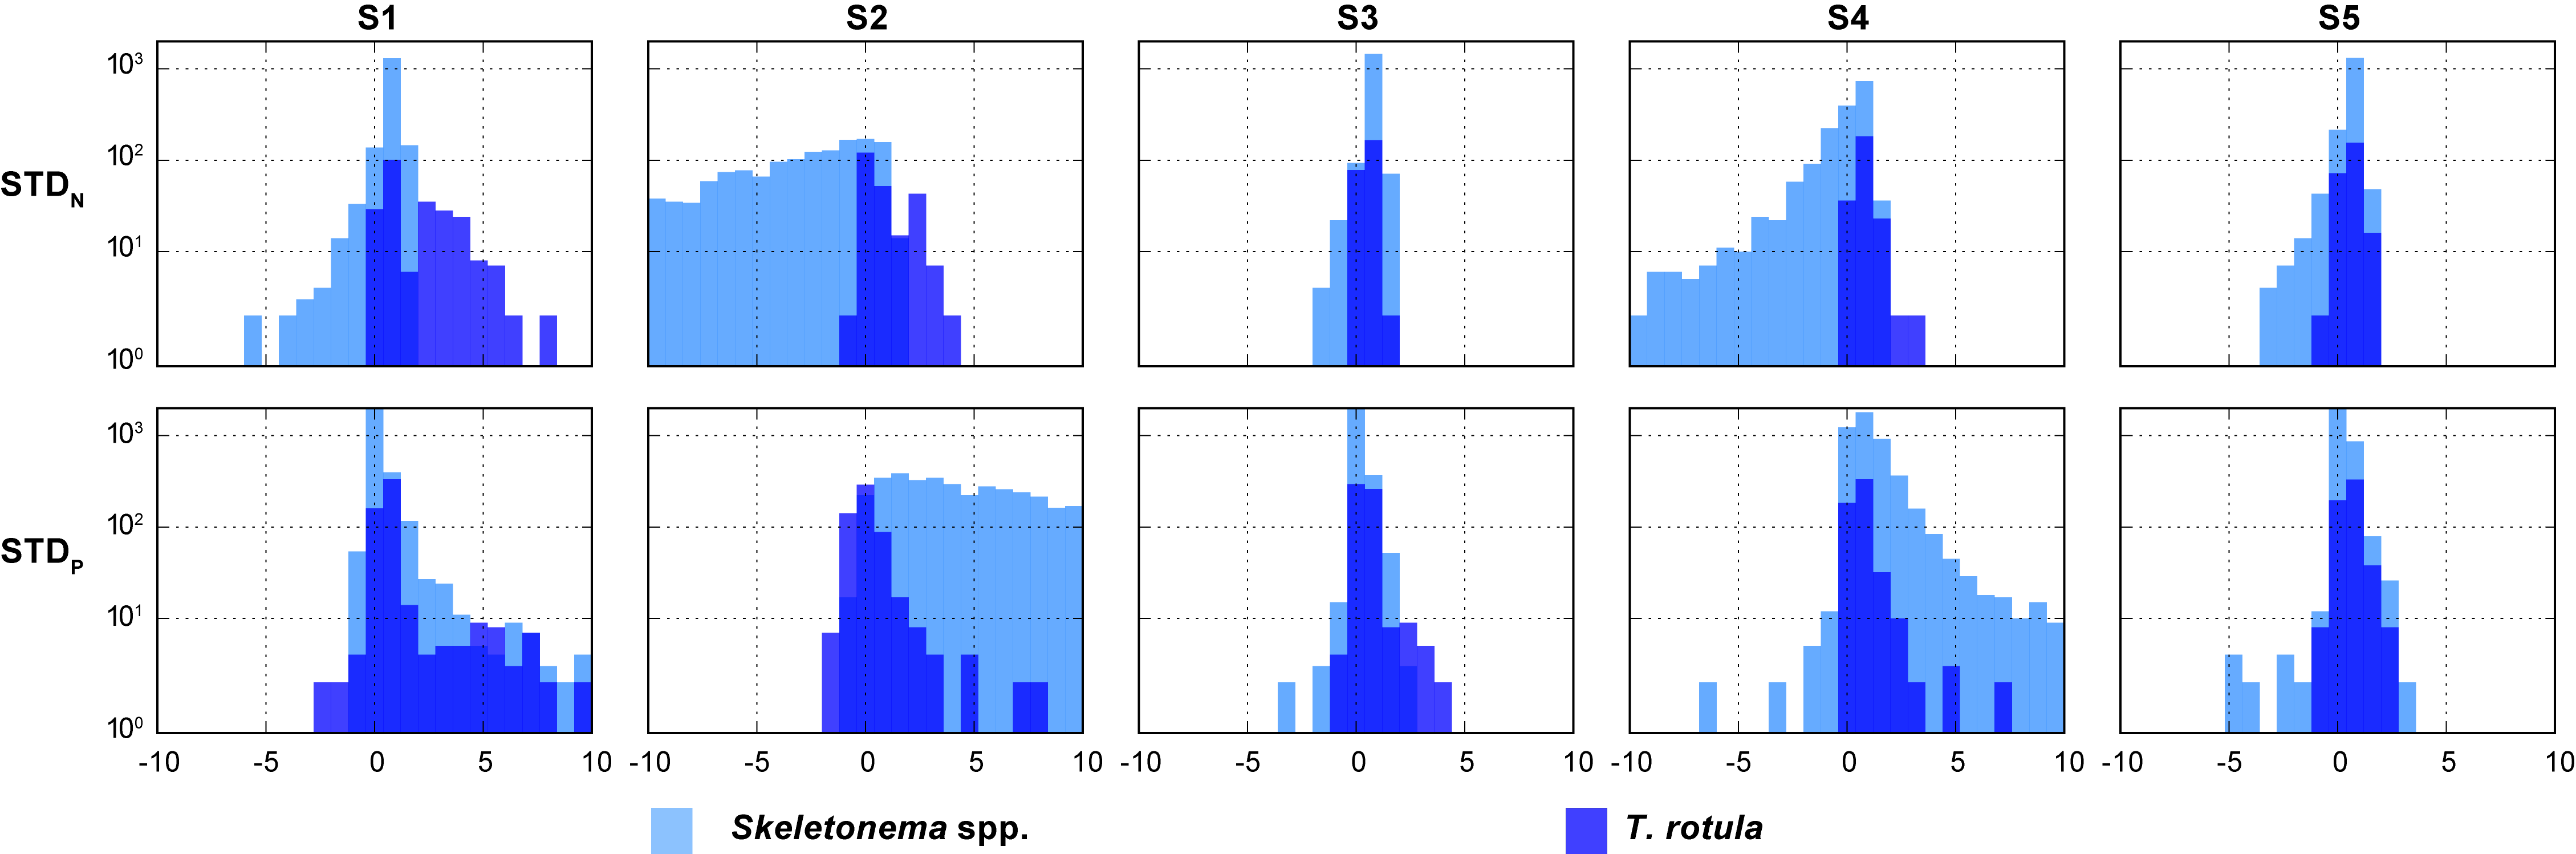
\includegraphics[width=1.3\textwidth]{Images/C3_STD_Histograms.png}
    	\caption[Distribution of $STD$ scores for N- and P-responsive genes]{The distribution of the standardized transcriptional differentiation scores for nitrogen and phosphorus, $STD_N$ and $STD_P$ was assessed for the N- and P-responsive genes, respectively for \textit{T. rotula}, dark blue, and \textit{Skeletonema} spp., light blue, across the five samples. The stable gene normalized counts ($SGNC$) of the N- and P-responsive genes (2-fold change, post$-p > 0.95$) was normalized to their expression in the like incubation experiments. A semi-log plot is used to show the distribution of gene counts between -10 and 10 for both of the organisms across the five samples.}
  	\label{fig:a3f9}
	\end{figure}
    \vfill        %%<----- and here
\end{landscape}



%%%% OLD FIGURES %%%%

%Supplemental Figure 10: Percentage of RR genes by quadrant

%\begin{figure}[h!]
%  \centering
    %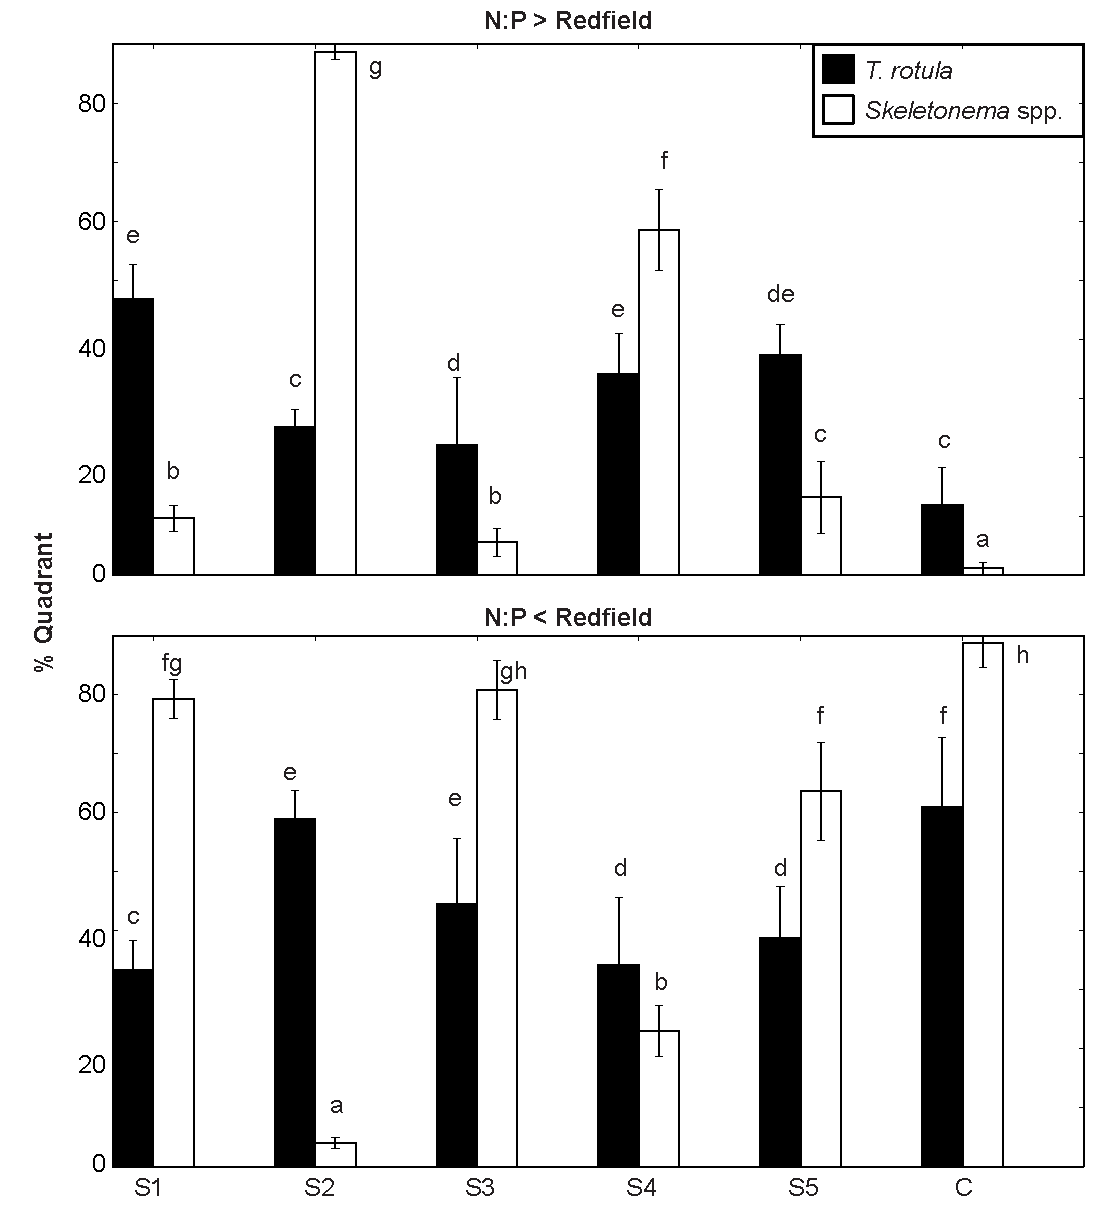
\includegraphics[width=1\textwidth]{Images/C3_SFigure10_BarGraph_Quadrant_2575_stats.pdf}
    %\caption[The percentage of identified nutrient responsive genes falling into the N:P > Redfield and N:P < Redfield quadrants with varried cutoffs]{The percentage of identified nutrient responsive genes falling into the N:P > Redfield and N:P < Redfield quadrants for \textit{T. rotula} and \textit{Skeletonema} spp.. The total number of genes falling into the N:P > Redfield quadrant ($STD_P > C$; $STD_N < C$, for $0.25 < C < 0.75$) and the N:P < Redfield quadrant ($STD_P$ < C; $STD_N > C$, for $0.25 < C < 0.75$). The value of C was varied over 10 different values and the average percentages of genes falling into each of the quadrants is depicted above based on the size of the circle at the median $STD_N$ and $STD_P$ for the genes in the quadrant. Similarity of data between species by quadrant was assessed using an analysis of variance (ANOVA) with a generalized linear model. The results from a post hoc Tukey test show the divergence of species across time ($p < 0.05$).}
 % \label{fig:a3f10}
%\end{figure}

%Supplemental Figure 11: Quadrant localization with varying stable reference genes

%\begin{figure}[p!]
%  \centering
%    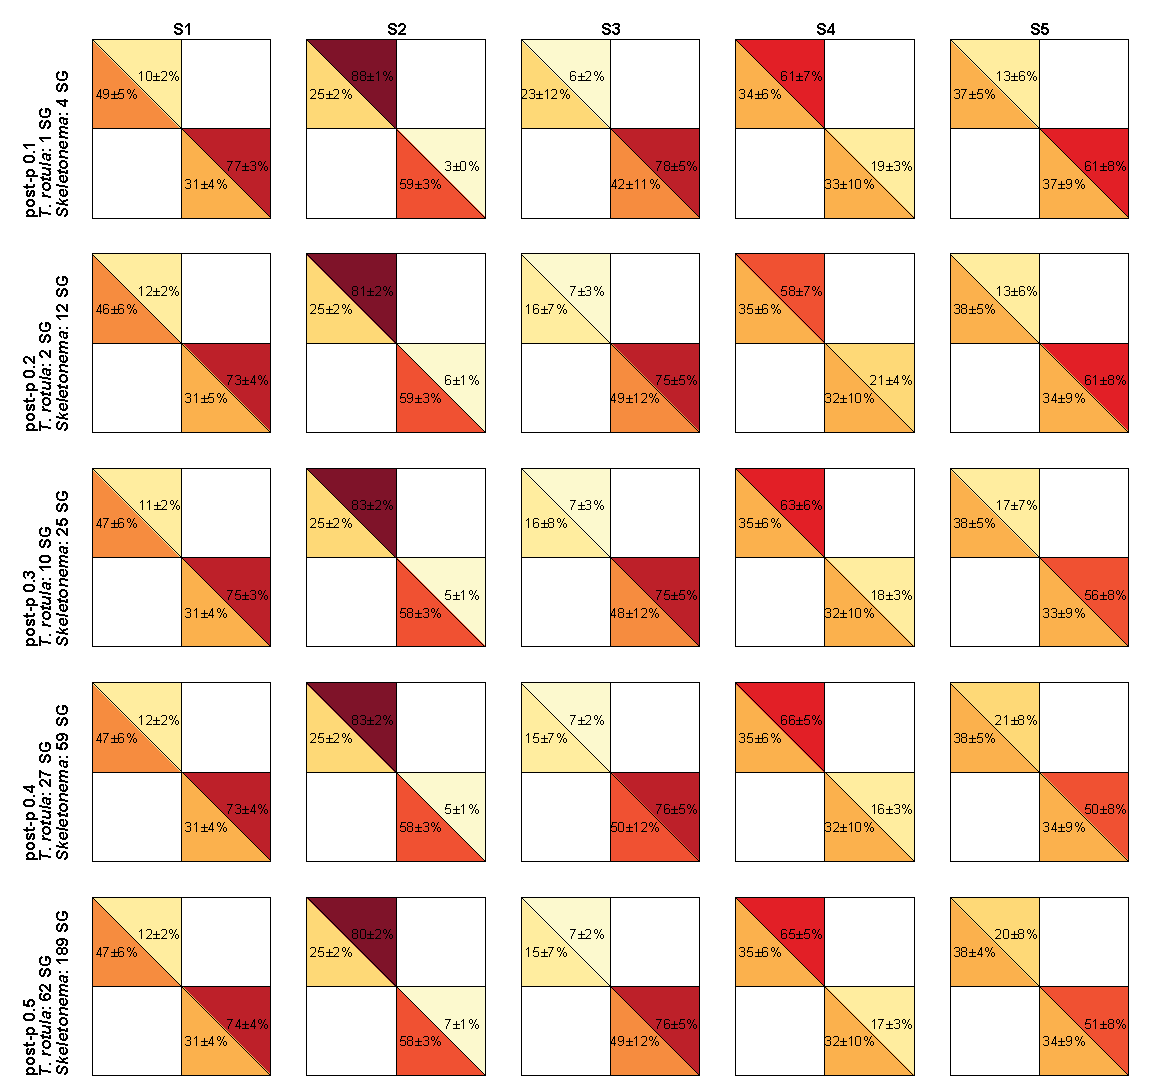
\includegraphics[width=1\textwidth]{Images/C3_SFigure11_Quadrant.pdf}
%    \caption[The impact of stable gene selction of quadrant localization]{The impact of stable gene selection on the quadrant localization of the resource responsive gene sets. The posterior probability cutoff used in the selection of stable genes was varied from 0.1 to 0.5 for a fold change of 1.25. The percentage of identified nutrient responsive genes falling into the N:P > Redfield and N:P < Redfield quadrants for \textit{T. rotula} and \textit{Skeletonema} spp. across the five sample points and five posterior probability values is depicted.}
%  \label{fig:a3f11}
%\end{figure}



\section{Supplemental Tables}

%Supplemental Table 1: library stats

\begin{table}[h!]
\centering
\caption[The total number of paired end reads after quality control and trimming and the percentage of reads mapping]{The total number of paired end reads after quality control and trimming and the percentage of reads mapping to the \textit{T. pseudonana} genome, \textit{T. rotula} transcriptome, and \textit{S. costatum} transcriptome.}
\label{tab:a3t1}
\newcolumntype{L}[1]{>{\raggedright\let\newline\\\arraybackslash\hspace{0pt}}m{#1}}
\label{my-label}
\begin{tabular}{lp{2cm}lll}
\multirow{2}{*}{Sample} & \multirow{2}{*}{\parbox{2cm}{Library Size (PE reads)}} & \multicolumn{3}{c}{\textbf{Representation in library}}             \\ 
                        &                                          & \textit{T. pseudonana} & \textit{T. rotula} & \textit{S. costatum} \\ \Xhline{2\arrayrulewidth}
S1                      & 89455034                                 & 2.98\%                 & 17.50\%            & 33.50\%              \\ \hline
S2                      & 64888267                                 & 0.41\%                 & 11.70\%            & 54.90\%              \\ \hline
S3                      & 103250243                                & 0.39\%                 & 7.30\%             & 9.00\%               \\ \hline
S4                      & 45370867                                 & 0.68\%                 & 8.80\%             & 8.30\%               \\ \hline
S5                      & 55061692                                 & 0.88\%                 & 10.40\%            & 11.20\%              \\ \hline
Ambient Control         & 51508197                                 & 0.27\%                 & 13.40\%            & 8.00\%               \\ \hline
+N                      & 58626239                                 & 0.43\%                 & 6.10\%             & 5.30\%               \\ \hline
-N                      & 44561851                                 & 0.41\%                 & 8.70\%             & 8.30\%               \\ \hline
+P                      & 51130364                                 & 0.29\%                 & 8.50\%             & 8.00\%               \\ \hline
-P                      & 58834022                                 & 0.40\%                 & 6.60\%             & 6.50\%               \\ \hline
\end{tabular}
\end{table}

%Supplememntal Table 2: nutrient concentrations used in incubations

\begin{table}[h!]
\centering
\caption[Nutrient concentrations used in nutrient amendment incubations. ]{Nutrient concentrations used in nutrient amendment incubations.}
\label{tab:a3t2}
\begin{tabular}{llllll}
            & \multicolumn{5}{c}{Treatment}                                        \\
Amendment   & Ambient Control & +N         & +P        & -N          & -P          \\\Xhline{2\arrayrulewidth}
Nitrate     & -               & $10 \mu M$ & -         & -           & $10 \mu M$  \\
Phosphate   & -               & -          & $3 \mu M$ & $3 \mu M$   & -           \\
Silica      & -               & -          & -         & $68 \mu M$  & $68 \mu M$  \\
Iron        & -               & -          & -         & $4.6 \mu M$ & $4.6 \mu M$ \\
Vitamin B12 & -               & -          & -         & f/5         & f/5        
\end{tabular}
\end{table}

%Supplememntal Table 3: nutrient concentrations used in incubations

\begin{table}[h!]
\centering
\caption[Mapping statistics for \textit{T. rotula} and \textit{S. costatum} transcriptomes]{Total number of contigs in the \textit{T. rotula} and \textit{S. costatum} transcriptomes and the number of genes in each of the differentially regulated and stable groupings.}
\label{tab:a3t3}
\newcolumntype{L}[1]{>{\raggedright\let\newline\\\arraybackslash\hspace{0pt}}m{#1}}
\begin{tabular}{L{3.5cm}ll}
\hline
                                                                       & \textit{\textbf{T. rotula}} & \textit{\textbf{S. costatum}} \\ \Xhline{2\arrayrulewidth}

Number of contigs in transcriptome                                     & 22362                       & 27665                         \\ \hline
Pass 2 TPM cutoff                                                      & 4318                        & 20921                         \\ \hline
Up in -P vs +P                                                         & 249                         & 4754                          \\ \hline
Down in -P vs +P                                                       & 335                         & 52                            \\ \hline
Up in -N vs +N                                                         & 196                         & 9                             \\ \hline
Down in -N vs +N                                                       & 49                          & 1631                          \\ \hline
All differentially regulated (2 fold change, post-$p > 0.95$) & 775                         & 5136                          \\ \hline
Stable genes (1.25 fold change, post-$p < 0.1$)                  & 1                           & 4                             \\ \hline
\end{tabular}
\end{table}

\clearpage

\section{Supplemental Data}

    \begin{DS3}
    
    \item \label{DS31}: Annotations based on KEGG Ontology for \textit{Skeletonema} spp. and \textit{T. rotula} transcriptomes. \href{http://www.pnas.org/content/suppl/2015/04/09/1421993112.DCSupplemental/pnas.1421993112.sd01.xlsx}{Data Sheet 3-1} can be downloaded from the online version of the manuscript of \citet{Alexander2015} through \href{http://www.pnas.org/content/112/17/E2182.full}{\textit{Proceedings of the National Academy of Sciences}}. 
    \item \label{DS32}: Relative expression in tags per million (TPM) for genes identified as differentially or stably expressed in nutrient incubations. \href{http://www.pnas.org/content/suppl/2015/04/09/1421993112.DCSupplemental/pnas.1421993112.sd02.xlsx}{Data Sheet 3-2} can be downloaded from the online version of the manuscript of \citet{Alexander2015} through \href{http://www.pnas.org/content/112/17/E2182.full}{\textit{Proceedings of the National Academy of Sciences}}. 
  
    \end{DS3}


